\documentclass{beamer}
\usepackage{graphicx}
\usepackage{xcolor}
\usepackage{tikz}

\usepackage{colortbl}     % 支持 \rowcolor
\usepackage[table]{xcolor}  % 增强颜色支持，特别是灰色背景
\usepackage{array}        % 增强表格功能（对齐方式等）
\usepackage{booktabs



% 自定义颜色
\definecolor{purpleblue}{RGB}{80, 80, 180}
\definecolor{lightgray}{RGB}{230, 230, 230}
\definecolor{novelPurple}{RGB}{98, 54, 255} 
\definecolor{darkgray}{RGB}{50, 50, 50}

% 主题设置
\usetheme{Madrid}  
\usecolortheme{dolphin} 

% 设置字体（移除 fontspec，确保 pdfLaTeX 兼容）
\setbeamerfont{title}{size=\Large,series=\bfseries}
\setbeamerfont{frametitle}{size=\LARGE,series=\bfseries}
\setbeamercolor{frametitle}{fg=white, bg=novelPurple}
\setbeamercolor{title}{fg=white, bg=purpleblue}

% 封面信息
\title[SAT Unit 4.4 ]{\textbf{SAT Unit 4.4\\ Circle }}
\author{\textbf{Jack Zeng}}
\institute{\textcolor{white}{\textbf{Novel Prep}}}
\date{\today} 

\begin{document}

% --- Title Slide ---
\begin{frame}
    \titlepage
    \vfill
    \begin{flushright}
        \textcolor{purpleblue}{\Huge \textbf{Novel Prep}}
    \end{flushright}
\end{frame}




\begin{frame}
    \begin{tikzpicture}[remember picture, overlay]
        % 设置浅色渐变背景
        \shade[top color=softPurple, bottom color=softGray] 
            (current page.north west) rectangle (current page.south east);
        
        % 添加高斯模糊光晕
        \fill[white, opacity=0.3] (current page.center) circle (4cm);
        
        % 主标题
        \node[align=center] at (current page.center) {
            {\Huge\bfseries\textcolor{purpleblue}{Novel Prep}} \\[0.5cm]
            {\Large\itshape\textcolor{lightText}{Excellence in SAT Prep}}
        };

        % 添加柔和光点（点缀）
        \foreach \x in {1,2,3,4,5} {
            \fill[purpleblue, opacity=0.2] (rand*10-5, rand*7-3.5) circle (0.1+\x*0.05);
        }

        ;
    \end{tikzpicture}
\end{frame}


\begin{frame}{Overview}
    \tableofcontents
\end{frame}





\begin{frame}
\section{Arc Length and Area of a Sector}
    \begin{tikzpicture}[remember picture, overlay]
        % 设置浅色渐变背景
        \shade[top color=softPurple, bottom color=softGray] 
            (current page.north west) rectangle (current page.south east);
        
        % 添加高斯模糊光晕
        \fill[white, opacity=0.3] (current page.center) circle (4cm);
        
        % 主标题
        \node[align=center] at (current page.center) {
            {\LARGE\bfseries\textcolor{purpleblue}{Arc Length and Area of a Sector}} \\[0.5cm]
            {\Large\itshape\textcolor{lightText}{Excellence in SAT Prep}}
        };

        % 添加柔和光点（点缀）
        \foreach \x in {1,2,3,4,5} {
            \fill[purpleblue, opacity=0.2] (rand*10-5, rand*7-3.5) circle (0.1+\x*0.05);
        }

        ;
    \end{tikzpicture}
\end{frame}


\begin{frame}{Arc Length of a Circle}
\small

\textbf{Arc Length Formula:}
\[
s = r\theta
\]
\textit{(where $s$ = arc length, $r$ = radius, $\theta$ = central angle in radians)}

\vspace{0.3cm}
\textbf{Example:}  
Find the arc length of a circle with:
\begin{itemize}
    \item Radius: $r = 6$
    \item Central angle: $\theta = 60^\circ = \frac{\pi}{3}$ radians
\end{itemize}

\vspace{0.2cm}
\[
s = r\theta = 6 \cdot \frac{\pi}{3} = 2\pi
\]

\vspace{0.3cm}
\textbf{SAT Tip:}  
Do not use this formula unless $\theta$ is in radians!

\end{frame}





\begin{frame}{Area of a Sector}
\small

\textbf{Definition:}  
A sector is a "pizza slice" portion of a circle.

\textbf{Formula (Radians):}
\[
\text{Area} = \frac{1}{2} r^2 \theta
\]

\vspace{0.3cm}
\textbf{Formula (Degrees):}
\[
\text{Area} = \frac{\theta^\circ}{360^\circ} \cdot \pi r^2
\]

\vspace{0.3cm}
\textbf{Example:}  
Find the area of a sector of a circle with radius 4 and angle $45^\circ$:

\[
\text{Area} = \frac{45}{360} \cdot \pi \cdot 4^2 = \frac{1}{8} \cdot 16\pi = 2\pi
\]

\vspace{0.2cm}
\textbf{SAT Reminder:} Be sure whether angle is in radians or degrees before using a formula.

\end{frame}


\begin{frame}{\textbf{Question: Arc Length and Central Angle}}

\begin{center}
    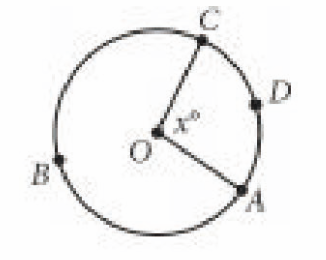
\includegraphics[width = 0.3\linewidth]{E39.png}
\end{center}

The circle above has center \( O \), the length of arc \( \widehat{ADC} \) is \( 5\pi \), and \( x = 100 \).  
What is the length of arc \( \widehat{ABC} \)?

\begin{itemize}
    \item[A.] \( 9\pi \)
    \item[B.] \( 13\pi \)
    \item[C.] \( 18\pi \)
    \item[D.] \( \frac{13}{2}\pi \)
\end{itemize}
\end{frame}


\begin{frame}{\textbf{Answer: Arc Length and Central Angle}}
We are told:
\begin{itemize}
    \item \( \text{Length of arc } \widehat{ADC} = 5\pi \)
    \item Central angle \( \angle AOC = x = 100^\circ \)
\end{itemize}

Since the entire circle represents \( 360^\circ \), the arc \( \widehat{ABC} \) must span:
\[
360^\circ - 100^\circ = 260^\circ
\]

Using the proportion of arc to full circle:
\[
\frac{260}{100} = \frac{\text{Length of } \widehat{ABC}}{\text{Length of } \widehat{ADC}} = \frac{L}{5\pi}
\Rightarrow L = 5\pi \cdot \frac{260}{100} = 13\pi
\]

\textbf{Correct Answer:} \fbox{\( \text{B. } 13\pi \)}
\end{frame}



\begin{frame}
\section{Properties of the Circle}
    \begin{tikzpicture}[remember picture, overlay]
        % 设置浅色渐变背景
        \shade[top color=softPurple, bottom color=softGray] 
            (current page.north west) rectangle (current page.south east);
        
        % 添加高斯模糊光晕
        \fill[white, opacity=0.3] (current page.center) circle (4cm);
        
        % 主标题
        \node[align=center] at (current page.center) {
            {\LARGE\bfseries\textcolor{purpleblue}{Properties of the Circle}} \\[0.5cm]
            {\Large\itshape\textcolor{lightText}{Excellence in SAT Prep}}
        };

        % 添加柔和光点（点缀）
        \foreach \x in {1,2,3,4,5} {
            \fill[purpleblue, opacity=0.2] (rand*10-5, rand*7-3.5) circle (0.1+\x*0.05);
        }

        ;
    \end{tikzpicture}
\end{frame}

\begin{frame}{Angles Inscribed in a Semicircle}
\small

\textbf{Theorem:}  
Any angle inscribed in a semicircle is a \textbf{right angle (90°)}.

\begin{itemize}
    \item If a triangle is inscribed in a circle and one side is the diameter, then the angle opposite that side is $90^\circ$.
\end{itemize}

\vspace{0.2cm}
\textbf{Example:}  
If triangle $ACB$ is inscribed in a circle and $AB$ is a diameter, then:
\[
\angle C = 90^\circ
\]

\begin{center}
    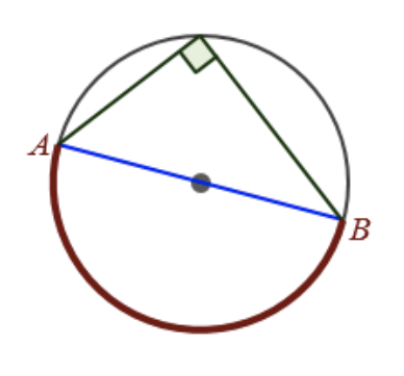
\includegraphics[width=0.3\linewidth]{E35.png}
\end{center}

\textbf{SAT Tip:}  
Look for a triangle with one side as a diameter — it’s a right triangle!

\end{frame}

\begin{frame}{Radius and Tangent Line}
\small

\textbf{Key Property:}  
The radius of a circle is \textbf{perpendicular} to the tangent line at the point of contact.

\begin{center}
    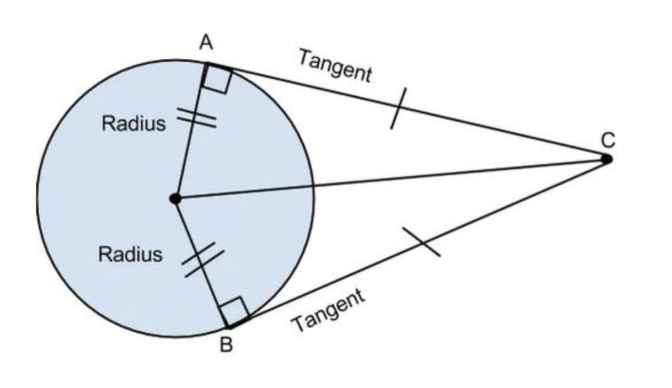
\includegraphics[width=0.4\linewidth]{E36.png}
\end{center}

\begin{itemize}
    \item Use this right angle in triangle questions.
    \item Often used in slope problems — if radius has slope $m$, tangent has slope $-\frac{1}{m}$.
\end{itemize}


\textbf{SAT Tip:}  
If the question mentions “tangent”, check for perpendicularity with radius.

\end{frame}

\begin{frame}{Radius Bisecting a Chord}
\small

\textbf{Theorem:}  
If a radius (or diameter) is perpendicular to a chord, it \textbf{bisects} the chord.

\vspace{0.2cm}
\[
\text{If } AB \perp OE,\ \text{then } AD = DB
\]

\begin{center}
    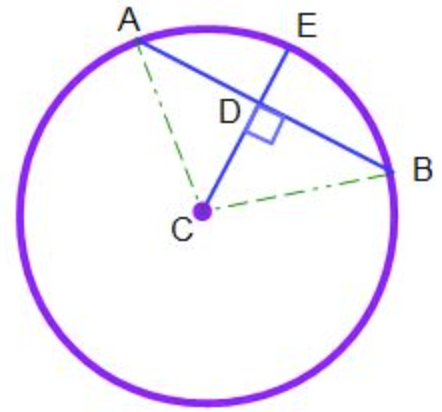
\includegraphics[width=0.20\linewidth]{E37.png}
\end{center}


\begin{itemize}
    \item Can be used to find missing lengths using right triangle properties.
    \item Also useful for coordinate geometry questions involving symmetry.
\end{itemize}

\textbf{Note:} The converse is also true — if a radius bisects a chord, it’s perpendicular.

\vspace{0.3cm}
\textbf{Useful for:} Midpoint formula, Pythagorean theorem, and algebraic proofs.

\end{frame}


\begin{frame}{\textbf{Question: Arc Length in Circle Geometry}}

\begin{center}
    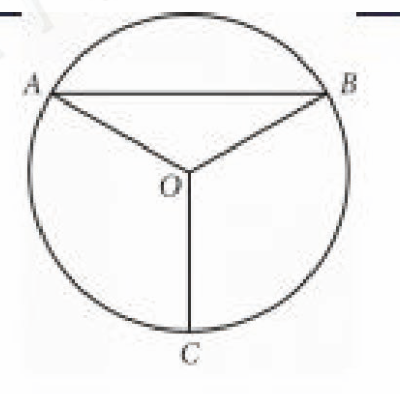
\includegraphics[width=0.3\linewidth]{E38.png}
\end{center}
Point \( O \) is the center of the circle above, and the measure of \( \angle OAB \) is \( 30^\circ \).  
If the length of \( \overline{OC} \) is \( 18 \), what is the length of arc \( \widehat{AB} \)?

\begin{itemize}
    \item[A.] \( 9\pi \)
    \item[B.] \( 12\pi \)
    \item[C.] \( 15\pi \)
    \item[D.] \( 18\pi \)
\end{itemize}
\end{frame}

\begin{frame}{\textbf{Answer: Arc Length in Circle Geometry}}
Since \( \angle OAB = 30^\circ \), the central angle for arc \( AB \) is \( 60^\circ \) (as it spans angle \( AOB \)).  
The radius is \( r = 18 \), so the circumference of the full circle is:
\[
C = 2\pi r = 2\pi(18) = 36\pi.
\]
The arc \( \widehat{AB} \) represents \( \frac{120^\circ}{360^\circ} = \frac{1}{3} \) of the full circle, so its length is:
\[
\frac{1}{3} \times 36\pi = 12\pi.
\]

\textbf{Correct Answer:} \fbox{\( 12\pi \)}  

\end{frame}



\begin{frame}
\section{Equation of a Circle in XY-Plane}
    \begin{tikzpicture}[remember picture, overlay]
        % 设置浅色渐变背景
        \shade[top color=softPurple, bottom color=softGray] 
            (current page.north west) rectangle (current page.south east);
        
        % 添加高斯模糊光晕
        \fill[white, opacity=0.3] (current page.center) circle (4cm);
        
        % 主标题
        \node[align=center] at (current page.center) {
            {\LARGE\bfseries\textcolor{purpleblue}{Equation of a Circle in XY-Plane}} \\[0.5cm]
            {\Large\itshape\textcolor{lightText}{Excellence in SAT Prep}}
        };

        % 添加柔和光点（点缀）
        \foreach \x in {1,2,3,4,5} {
            \fill[purpleblue, opacity=0.2] (rand*10-5, rand*7-3.5) circle (0.1+\x*0.05);
        }

        ;
    \end{tikzpicture}
\end{frame}



\begin{frame}{Equation of a Circle (Coordinate Plane)}
\small

\textbf{Standard Form:}
\[
(x - h)^2 + (y - k)^2 = r^2
\]

\textbf{Where:}
\begin{itemize}
    \item $(h, k)$ is the center,
    \item $r$ is the radius.
\end{itemize}

\vspace{0.2cm}
\textbf{Example:}  
Circle with center $(3, -2)$ and radius $5$:
\[
(x - 3)^2 + (y + 2)^2 = 25
\]

\textbf{SAT Skills:}
\begin{itemize}
    \item Completing the square to rewrite equations.
    \item Identify center and radius from expanded forms.
\end{itemize}

\end{frame}



\begin{frame}{Completing the Square to Find Circle Equation}
\small

\textbf{Given:}  
\[
x^2 + y^2 - 6x + 8y + 9 = 0
\]

\vspace{0.2cm}
\textbf{Steps:}
\begin{enumerate}
    \item Group $x$ and $y$ terms:
    \[
    (x^2 - 6x) + (y^2 + 8y) = -9
    \]
    \item Complete the square:
    \[
    (x - 3)^2 - 9 + (y + 4)^2 - 16 = -9
    \]
    \item Simplify:
    \[
    (x - 3)^2 + (y + 4)^2 = 16
    \]
\end{enumerate}

\vspace{0.2cm}
\textbf{Final Answer:} Center = $(3, -4)$, Radius = $4$

\textbf{SAT Tip:} Always isolate constants and complete square carefully on both $x$ and $y$ terms.

\end{frame}

\begin{frame}{\textbf{Question: Completing the Square }}

The graph of the equation 
\[
x^2 + x + y^2 + y = \frac{199}{2}
\]
in the \(xy\)-plane is a circle. What is the length of the circle’s radius?
\end{frame}


\begin{frame}{\textbf{Answer: Completing the Square – Radius of a Circle}}
\small
To convert the given equation to the standard form of a circle, complete the square for both \(x\) and \(y\):

\[
x^2 + x + y^2 + y = \frac{199}{2}
\]

Complete the square:

\[
x^2 + x = \left(x + \frac{1}{2}\right)^2 - \frac{1}{4}, \quad y^2 + y = \left(y + \frac{1}{2}\right)^2 - \frac{1}{4}
\]

So,

\[
\left(x + \frac{1}{2}\right)^2 - \frac{1}{4} + \left(y + \frac{1}{2}\right)^2 - \frac{1}{4} = \frac{199}{2}
\]

\[
\left(x + \frac{1}{2}\right)^2 + \left(y + \frac{1}{2}\right)^2 = \frac{199}{2} + \frac{1}{2} = \frac{200}{2} = 100
\]

Thus, the radius is:

\[
r = \sqrt{100} = 10
\]
\end{frame}



\begin{frame}
\section{Properties of the Circle}
    \begin{tikzpicture}[remember picture, overlay]
        % 设置浅色渐变背景
        \shade[top color=softPurple, bottom color=softGray] 
            (current page.north west) rectangle (current page.south east);
        
        % 添加高斯模糊光晕
        \fill[white, opacity=0.3] (current page.center) circle (4cm);
        
        % 主标题
        \node[align=center] at (current page.center) {
            {\Huge\bfseries\textcolor{purpleblue}{Practices}} \\[0.5cm]
            {\Large\itshape\textcolor{lightText}{Excellence in SAT Prep}}
        };

        % 添加柔和光点（点缀）
        \foreach \x in {1,2,3,4,5} {
            \fill[purpleblue, opacity=0.2] (rand*10-5, rand*7-3.5) circle (0.1+\x*0.05);
        }

        ;
    \end{tikzpicture}
\end{frame}


\begin{frame}{Equation of a Circle}
\textbf{Question:}  
The center of a circle in the \(xy\)-plane is at \((1, -1)\) and the point \((-5, 7)\) lies on the circle. Which of the following equations represents this circle?
\begin{itemize}
    \item[A] \( (x + 1)^2 + (y - 1)^2 = 10 \)
    \item[B] \( (x - 1)^2 + (y + 1)^2 = 10 \)
    \item[C] \( (x + 1)^2 + (y - 1)^2 = 100 \)
    \item[D] \( (x - 1)^2 + (y + 1)^2 = 100 \)
\end{itemize}
\end{frame}

\begin{frame}{Solution}
\textbf{Solution:}  
- The center is at \((1, -1)\).
- Find the radius using the distance formula:
\[
r = \sqrt{(-5 - 1)^2 + (7 - (-1))^2} = \sqrt{(-6)^2 + (8)^2} = \sqrt{36 + 64} = \sqrt{100} = 10
\]
- The circle’s equation is:
\[
(x - 1)^2 + (y + 1)^2 = 100
\]
\[
\boxed{\text{Answer: D}}
\]
\end{frame}


\begin{frame}{Circles in the \(xy\)-Plane}
\textbf{Question:}  
In the \(xy\)-plane, circle \(A\) is defined by the equation \((x - 3)^2 + (y - 4)^2 = 16\), and circle \(B\) is defined by the equation \((x - 3)^2 + (y - 4)^2 = n\), where \(n\) is a constant. The diameter of circle \(B\) is 48 units longer than the diameter of circle \(A\). What is the value of \(n\)?
\end{frame}

\begin{frame}{Solution}
\textbf{Solution:}
\begin{itemize}
    \item Circle \(A\):
    \[
    r_A = \sqrt{16} = 4 \quad \Rightarrow \quad d_A = 2 \times 4 = 8
    \]
    \item Circle \(B\):
    \[
    d_B = d_A + 48 = 8 + 48 = 56 \quad \Rightarrow \quad r_B = 28
    \]
    \item Therefore:
    \[
    r_B^2 = 28^2 = 784
    \]
    Hence:
    \[
    \boxed{n = 784}
    \]
\end{itemize}
\end{frame}

\begin{frame}{Circle in the \(xy\)-Plane}
\textbf{Question:}  
The given equation represents a circle in the \(xy\)-plane:
\[
x^2 + y^2 + 7x + y = -\frac{7}{2}
\]
What is the length of the radius of the circle?
\end{frame}

\begin{frame}{Solution}
\scriptsize

\begin{itemize}
    \item Start with:
    \[
    x^2 + 7x + y^2 + y = -\frac{7}{2}
    \]
    \item Complete the square:
    \[
    x^2 + 7x \rightarrow x^2 + 7x + \left(\frac{7}{2}\right)^2 = \left(x + \frac{7}{2}\right)^2 - \frac{49}{4}
    \]
    \[
    y^2 + y \rightarrow y^2 + y + \left(\frac{1}{2}\right)^2 = \left(y + \frac{1}{2}\right)^2 - \frac{1}{4}
    \]
    \item Combine:
    \[
    \left(x + \frac{7}{2}\right)^2 - \frac{49}{4} + \left(y + \frac{1}{2}\right)^2 - \frac{1}{4} = -\frac{7}{2}
    \]
    \item Bring constants to the right:
    \[
    \left(x + \frac{7}{2}\right)^2 + \left(y + \frac{1}{2}\right)^2 = -\frac{7}{2} + \frac{49}{4} + \frac{1}{4}
    \]
    \[
    = -\frac{7}{2} + \frac{50}{4}
    \]
    \[
    = -\frac{14}{4} + \frac{50}{4} = \frac{36}{4} = 9
    \]
    \item Therefore:
    \[
    r = \sqrt{9} = \boxed{3}
    \]
\end{itemize}
\end{frame}


\begin{frame}{Triangle DEF}
\textbf{Question:}  
In the \(xy\)-plane, a circle has center \(D\) with coordinates \((m,16)\), where \(m\) is a constant. Points \(E\) and \(F\) lie on the circle. Point \(E\) lies on the circle and has coordinates \((m+4\sqrt{10},34)\), and point \(F\) has coordinates \((n,16)\), where \(n\) is a constant greater than \(m\). What is the area, in square units, of triangle \(DEF\)?

\begin{itemize}
    \item[A] \(198\)
    \item[B] \(72\sqrt{10}\)
    \item[C] \(242\)
    \item[D] \(99\sqrt{10}\)
\end{itemize}
\end{frame}

\begin{frame}{Solution}
\textbf{Solution:}
\begin{itemize}

    \item 
    \[
    \boxed{198}.
    \]
\end{itemize}
\end{frame}


\begin{frame}{Tangent Line and Circle}
\textbf{Question:}  
A circle in the \(xy\)-plane has the equation 
\[
(x-2)^2 + (y-2)^2 = 25.
\] 
Line \(m\) is tangent to this circle at the point \((5,6)\). What is the \(y\)-coordinate of the \(y\)-intercept of line \(m\)?
\end{frame}

\begin{frame}{Solution}
\footnotesize
\textbf{Solution:}
\begin{itemize}
    \item The center of the circle is at \((2,2)\), and the radius is \(5\).
    \item The tangent line at point \((5,6)\) is perpendicular to the radius at that point.
    \item The slope of the radius is:
    \[
    \frac{6-2}{5-2} = \frac{4}{3}.
    \]
    \item Therefore, the slope of line \(m\) is the negative reciprocal:
    \[
    -\frac{3}{4}.
    \]
    \item Using the point-slope form:
    \[
    y - 6 = -\frac{3}{4}(x - 5).
    \]
    \item Setting \(x = 0\) to find the \(y\)-intercept:
    \[
    y = 6 + \frac{15}{4} = \frac{24}{4} + \frac{15}{4} = \frac{39}{4}.
    \]
    \item Therefore:
    \[
    \boxed{\frac{39}{4}}.
    \]
\end{itemize}
\end{frame}








\begin{frame}{}

    \begin{tikzpicture}[remember picture, overlay]

        \shade[top color=novelPurple!40, bottom color=white]
            (current page.north west) rectangle (current page.south east);

    
        \fill[white, opacity=0.15] (current page.center) circle (5cm);

        \foreach \x in {1,2,3,4,5} {
            \fill[novelPurple, opacity=0.12] (rand*10-5, rand*7-3.5) circle (0.1+\x*0.05);
        }
    \end{tikzpicture}

    \centering
    \vspace{5em}

    {\Huge \textbf{\textcolor{novelPurple}{Thank You!}}} \\[1em]
    {\large \textcolor{gray}{We appreciate your time and focus.}} \\[3em]

    {\LARGE \textbf{\textcolor{novelPurple}{\textsf{Novel Prep}}}}

    \vfill
\end{frame}











\end{document}